\documentclass{article}
\usepackage{amsmath}
\usepackage{amssymb}
\usepackage{amsthm}
\usepackage{listings}
\usepackage{xcolor}
\usepackage{graphicx}

\definecolor{codegreen}{rgb}{0,0.6,0}
\definecolor{codegray}{rgb}{0.5,0.5,0.5}
\definecolor{codepurple}{rgb}{0.58,0,0.82}
\definecolor{backcolour}{rgb}{0.95,0.95,0.92}

\lstdefinestyle{mystyle}{
    backgroundcolor=\color{backcolour},   
    commentstyle=\color{codegreen},
    keywordstyle=\color{magenta},
    numberstyle=\tiny\color{codegray},
    stringstyle=\color{codepurple},
    basicstyle=\ttfamily\footnotesize,
    breakatwhitespace=false,         
    breaklines=true,                 
    captionpos=b,                    
    keepspaces=true,                 
    numbers=left,                    
    numbersep=5pt,                  
    showspaces=false,                
    showstringspaces=false,
    showtabs=false,                  
    tabsize=4,
    language=Python
}
\lstset{style=mystyle}

\title{EEE 554 Homework 2}
\author{Chaofei Guo (Student ID: 1237382330, ASURITE: chaofeig)}
\date{}

\begin{document}
\maketitle

\section*{Problem 1 (Problem 5-35, page 166)}
\textbf{Problem Statement:}
(Chernoff bound)
(a) Show that for any $\alpha > 0$ and for any real $s$,
\[ P\{e^{sx} \ge \alpha\} \le \frac{\Phi(s)}{\alpha} \quad \text{where } \Phi(s) = E[e^{sx}] \]
(b) For any $A$,
\begin{align*}
P\{x \ge A\} &\le e^{-sA}\Phi(s) \quad \text{for } s > 0 \\
P\{x \le A\} &\le e^{-sA}\Phi(s) \quad \text{for } s < 0
\end{align*}

\begin{proof}[Solution]
	\textbf{Part (a)}\\
	Let $y = e^{sx}$. Since the exponential function is strictly positive, $y$ is a non-negative random variable ($y > 0$).
	From Markov's inequality, for any non-negative random variable $y$ and constant $\alpha > 0$:
	\[ P\{y \ge \alpha\} \le \frac{E[y]}{\alpha} \]
	Substituting $y = e^{sx}$ into the inequality yields:
	\[ P\{e^{sx} \ge \alpha\} \le \frac{E[e^{sx}]}{\alpha} = \frac{\Phi(s)}{\alpha} \]
	
	\textbf{Part (b)}\\
	For $s > 0$, the function $g(x) = e^{sx}$ is strictly monotonically increasing. Thus, the event $\{x \ge A\}$ is exactly equivalent to the event $\{e^{sx} \ge e^{sA}\}$.
	Using the result from Part (a) with $\alpha = e^{sA}$:
	\[ P\{x \ge A\} = P\{e^{sx} \ge e^{sA}\} \le \frac{\Phi(s)}{e^{sA}} = e^{-sA}\Phi(s) \]
	
	For $s < 0$, the function $g(x) = e^{sx}$ is strictly monotonically decreasing. Multiplying the inequality $x \le A$ by a negative number $s$ we get $sx \ge sA$. And $e^{sx} \ge e^{sA}$, so the event $\{x \le A\}$ is exactly equivalent to the event $\{e^{sx} \ge e^{sA}\}$.
	Again, using the result from Part (a) with $\alpha = e^{sA}$:
	\[ P\{x \le A\} = P\{e^{sx} \ge e^{sA}\} \le \frac{\Phi(s)}{e^{sA}} = e^{-sA}\Phi(s) \]
\end{proof}

\vspace{1cm}

\section*{Problem 2}
\textbf{Problem Statement:}
The RV $n$ is normal with mean zero and variance one. Under $H_0$, $x=n$. Under $H_1$, $x=s+n$ where $s \ge 0$.
(a) If $P(H_0)=P(H_1)$, for what range of $x$ should a hypothesis test decide in favor of $H_1$? In terms of $s$, what are $P_d$, $P_f$, and $P_e$ for this test?
(b) Take $s=1$ and find $P_d$ and $P_f$ in terms of the ratio $T=P(H_0)/P(H_1)$. Use these expressions to sketch the ROC curve.

\begin{proof}[Solution]
	\textbf{Part (a)}\\
	The conditional PDFs of the observation $x$ under the two hypotheses are:
	\begin{align*}
		f_x(x|H_0) &= \frac{1}{\sqrt{2\pi}} e^{-x^2/2} \\
		f_x(x|H_1) &= \frac{1}{\sqrt{2\pi}} e^{-(x-s)^2/2}
	\end{align*}
	The likelihood ratio test decides $H_1$ if:
	\[
		\frac{f_x(x|H_1)}{f_x(x|H_0)} > \frac{P(H_0)}{P(H_1)}
	\]
	Since $P(H_0) = P(H_1)$, the threshold is 1. Substituting the PDFs:
	\[
		\exp\left( -\frac{(x-s)^2}{2} + \frac{x^2}{2} \right) > 1 \implies \exp\left( xs - \frac{s^2}{2} \right) > 1
	\]
	Taking the natural logarithm of both sides:
	\[
		xs - \frac{s^2}{2} > 0 \implies x > \frac{s}{2} \quad \text{(since } s \ge 0 \text{)}
	\]
	Thus, the test should decide in favor of $H_1$ for $x \in \left(\frac{s}{2}, \infty\right)$.
	
	Let $Q(z) = \int_z^\infty \frac{1}{\sqrt{2\pi}} e^{-u^2/2} du$:
	\begin{itemize}
	    \item \textbf{Probability of False Alarm ($P_f$):} 
	    \[ P_f = P(x > s/2 \mid H_0) = P(n > s/2) = Q\left(\frac{s}{2}\right) \]
	    \item \textbf{Probability of Detection ($P_d$):} 
	    \[ P_d = P(x > s/2 \mid H_1) = P(s+n > s/2) = P(n > -s/2) = Q\left(-\frac{s}{2}\right) = 1 - Q\left(\frac{s}{2}\right) \]
	    \item \textbf{Probability of Error ($P_e$):}
	    \begin{align*}
	        P_e &= P(H_0)P_f + P(H_1)(1 - P_d) \\
	        &= \frac{1}{2}Q\left(\frac{s}{2}\right) + \frac{1}{2}\left(1 - \left[1 - Q\left(\frac{s}{2}\right)\right]\right) = Q\left(\frac{s}{2}\right)
	    \end{align*}
	\end{itemize}
	
	\vspace{0.5cm}
	\textbf{Part (b)}\\
	Let $s=1$. The threshold is $T = P(H_0)/P(H_1)$. The decision rule becomes:
	\[
		x - \frac{1^2}{2} > \ln T \implies x > \ln T + \frac{1}{2}
	\]
	Let $\gamma = \ln T + 1/2$ be the decision threshold.
	\begin{align*}
		P_f &= P(x > \gamma \mid H_0) = Q(\gamma) \implies \gamma = Q^{-1}(P_f) \\
		P_d &= P(x > \gamma \mid H_1) = P(1+n > \gamma) = P(n > \gamma - 1) = Q(\gamma - 1)
	\end{align*}
	Substituting $\gamma$, we obtain the ROC curve equation:
	\[
		P_d = Q\left(Q^{-1}(P_f) - 1\right)
	\]
	\end{proof}

\vspace{1cm}

\section*{Problem 3}
\textbf{Problem Statement:}
Under $H_0$, $x$ has conditional PDF $f_x(x|H_0)$. Under $H_1$, its conditional PDF is $f_x(x|H_1)$. Show that the Bayesian decision rule
\[
	\text{Choose } H_1 \text{ if } \frac{f_x(x|H_1)}{f_x(x|H_0)} > \frac{P(H_0)}{P(H_1)}
\]
minimizes the probability of error $P_e$.

\begin{proof}[Solution]
	The total probability of error $P_e$ is the sum of the probabilities of making a false alarm (choosing $H_1$ when $H_0$ is true) and a miss (choosing $H_0$ when $H_1$ is true). Let $R_1$ be the decision region for $H_1$ and $R_0$ be the decision region for $H_0$. 
	\begin{align*}
		P_e &= P(H_0) P(x \in R_1 \mid H_0) + P(H_1) P(x \in R_0 \mid H_1) \\
		&= P(H_0) \int_{R_1} f_x(x|H_0) dx + P(H_1) \int_{R_0} f_x(x|H_1) dx
	\end{align*}
	Since $R_0$ and $R_1$ partition the sample space, $\int_{R_0} f_x(x|H_1) dx = 1 - \int_{R_1} f_x(x|H_1) dx$. Substitute this into the equation:
	\begin{align*}
		P_e &= P(H_0) \int_{R_1} f_x(x|H_0) dx + P(H_1) \left(1 - \int_{R_1} f_x(x|H_1) dx\right) \\
		&= P(H_1) + \int_{R_1} \left[ P(H_0) f_x(x|H_0) - P(H_1) f_x(x|H_1) \right] dx
	\end{align*}
	To minimize $P_e$, we must minimize the integral. This is achieved by including a point $x$ in the region $R_1$ if and only if the integrand evaluated at $x$ is negative:
	\[
		P(H_0) f_x(x|H_0) - P(H_1) f_x(x|H_1) < 0
	\]
	Rearranging the terms yields the optimal decision rule:
	\[
		P(H_1) f_x(x|H_1) > P(H_0) f_x(x|H_0) \implies \frac{f_x(x|H_1)}{f_x(x|H_0)} > \frac{P(H_0)}{P(H_1)}
	\]
	\end{proof}

\vspace{1cm}

\section*{Problem 4}
\textbf{Problem Statement:}
The joint PDF of $x_1$ and $x_2$ is $f_{x_1,x_2}(x_1,x_2) = a$ if $x_1 \ge 0, x_2 \ge 0$ and $x_1+x_2 \le 1$, and $0$ otherwise.
(a) Find the value of $a$.
(b) Calculate $E[x_1]$, $\text{var}(x_1)$, and $\text{cov}(x_1,x_2)$.

\begin{proof}[Solution]
	\textbf{Part (a)}\\
	CDF must equal 1.
	\[
		\iint f(x_1, x_2) dx_1 dx_2 = a \times \text{Area} = a \left(\frac{1}{2}\right) = 1 \implies a = 2
	\]

	\textbf{Part (b)}\\
	First, we find the marginal PDF of $x_1$:
	\[
		f_{x_1}(x_1) = \int_0^{1-x_1} 2 \,dx_2 = 2(1 - x_1), \quad 0 \le x_1 \le 1
	\]
	Now we calculate the moments for $x_1$:
	\begin{align*}
		E[x_1] &= \int_0^1 x_1 \cdot 2(1-x_1) dx_1 = 2 \left[ \frac{x_1^2}{2} - \frac{x_1^3}{3} \right]_0^1 = 2\left(\frac{1}{2} - \frac{1}{3}\right) = \frac{1}{3} \\
		E[x_1^2] &= \int_0^1 x_1^2 \cdot 2(1-x_1) dx_1 = 2 \left[ \frac{x_1^3}{3} - \frac{x_1^4}{4} \right]_0^1 = 2\left(\frac{1}{3} - \frac{1}{4}\right) = \frac{1}{6} \\
		\text{var}(x_1) &= E[x_1^2] - (E[x_1])^2 = \frac{1}{6} - \left(\frac{1}{3}\right)^2 = \frac{1}{6} - \frac{1}{9} = \frac{1}{18}
	\end{align*}
	By symmetry, $E[x_2] = \frac{1}{3}$. Next, we calculate the cross-moment $E[x_1 x_2]$:
	\begin{align*}
		E[x_1 x_2] &= \int_0^1 \int_0^{1-x_1} x_1 x_2 (2) dx_2 dx_1 = \int_0^1 2 x_1 \left[ \frac{x_2^2}{2} \right]_0^{1-x_1} dx_1 \\
		&= \int_0^1 x_1 (1 - 2x_1 + x_1^2) dx_1 = \int_0^1 (x_1 - 2x_1^2 + x_1^3) dx_1 \\
		&= \frac{1}{2} - \frac{2}{3} + \frac{1}{4} = \frac{1}{12}
	\end{align*}
	Finally, the covariance is:
	\[
		\text{cov}(x_1, x_2) = E[x_1 x_2] - E[x_1]E[x_2] = \frac{1}{12} - \left(\frac{1}{3}\right)\left(\frac{1}{3}\right) = \frac{3}{36} - \frac{4}{36} = -\frac{1}{36}
	\]
\end{proof}

\vspace{1cm}

\section*{Problem 5 (Problem 5-12, page 165)}
\textbf{Problem Statement:}
The random variable $x$ is uniform in the interval $(-2\pi, 2\pi)$. Find $f_y(y)$ if (a) $y = x^3$, and (b) $y = x^4$.
and (c) $y = 2 \sin(3x + 40^\circ)$: \\ 

\begin{proof}[Solution]
	Given $x \sim U(-2\pi, 2\pi)$, its probability density function is:
	\[
		f_x(x) = \frac{1}{4\pi}, \quad -2\pi < x < 2\pi
	\]
	
	\textbf{Part (a)} $y = x^3$: \\
	The transformation is strictly monotonically increasing. The inverse is $x = y^{1/3}$.
	The derivative is $\frac{dx}{dy} = \frac{1}{3}y^{-2/3}$.
	Using the fundamental theorem for functions of one random variable:
	\[
		f_y(y) = f_x(x) \left| \frac{dx}{dy} \right| = \frac{1}{4\pi} \left| \frac{1}{3} y^{-2/3} \right| = \frac{1}{12\pi y^{2/3}}
	\]
	Since $x \in (-2\pi, 2\pi)$, the range of $y$ is $(-8\pi^3, 8\pi^3)$. Thus:
	\[
		f_y(y) = \frac{1}{12\pi y^{2/3}}, \quad -8\pi^3 < y < 8\pi^3
	\]
	
	\textbf{Part (b)} $y = x^4$: \\
	For $y \in (0, 16\pi^4)$, the equation $y = x^4$ has two real roots: $x_1 = y^{1/4}$ and $x_2 = -y^{1/4}$.
	The derivative magnitude for each root is $\left| \frac{dx}{dy} \right| = \frac{1}{4} y^{-3/4}$.
	Summing the contributions from both roots:
	\[
		f_y(y) = \frac{f_x(x_1)}{|g'(x_1)|} + \frac{f_x(x_2)}{|g'(x_2)|} = \frac{1/4\pi}{4y^{3/4}} + \frac{1/4\pi}{4y^{3/4}} = \frac{1}{8\pi y^{3/4}}
	\]
	Thus:
	\[
		f_y(y) = \frac{1}{8\pi y^{3/4}}, \quad 0 < y < 16\pi^4
	\]

	\textbf{Part (c)} $y = 2 \sin(3x + 40^\circ)$: \\
The interval of $x$ is $(-2\pi, 2\pi)$, which has a length of $4\pi$. The argument of the sine function, $3x + 40^\circ$, covers an interval of $3 \times 4\pi = 12\pi$. Since the period of a sine wave is $2\pi$, this range covers exactly 6 full periods.
For any given $y \in (-2, 2)$, the equation $y = 2 \sin(3x + 40^\circ)$ has exactly $6 \times 2 = 12$ roots in the interval.

The derivative of the transformation is:
\[
    g'(x) = \frac{dy}{dx} = 6 \cos(3x + 40^\circ)
\]
In terms of $y$, the magnitude of the derivative at each root is:
\[
    |g'(x)| = 6 \sqrt{1 - \sin^2(3x + 40^\circ)} = 6 \sqrt{1 - \left(\frac{y}{2}\right)^2} = 3\sqrt{4 - y^2}
\]
Applying the fundamental theorem for 12 roots:
\[
    f_y(y) = \sum_{i=1}^{12} \frac{f_x(x_i)}{|g'(x_i)|} = 12 \times \left( \frac{1/4\pi}{3\sqrt{4 - y^2}} \right) = \frac{1}{\pi\sqrt{4 - y^2}}
\]
The range of $y$ is determined by the amplitude, which is $(-2, 2)$. Thus:
\[
    f_y(y) = \frac{1}{\pi\sqrt{4 - y^2}}, \quad -2 < y < 2
\]
\end{proof}

\vspace{1cm}

\section*{Problem 6 (Alternative Transformation)}
\textbf{Problem Statement:}
Let $x$ be a chi-square random variable with $n$ degrees of freedom. Find the p.d.f. of $y = x^2$.

\begin{proof}[Solution]
	The p.d.f. of $x \sim \chi^2(n)$ is:
	\[
		f_x(x) = \frac{1}{2^{n/2}\Gamma(n/2)} x^{n/2-1} e^{-x/2}, \quad x > 0
	\]
	Given the transformation $y = x^2$, the inverse transformation for $x > 0$ is $x = \sqrt{y}$.
	The derivative is:
	\[
		\frac{dx}{dy} = \frac{d}{dy}(y^{1/2}) = \frac{1}{2}y^{-1/2}
	\]
	Applying the transformation theorem:
	\begin{align*}
		f_y(y) &= f_x(\sqrt{y}) \left| \frac{dx}{dy} \right| \\
		&= \frac{1}{2^{n/2}\Gamma(n/2)} (\sqrt{y})^{n/2-1} e^{-\sqrt{y}/2} \cdot \frac{1}{2}y^{-1/2} \\
		&= \frac{1}{2^{n/2+1}\Gamma(n/2)} y^{\frac{n}{4}-\frac{1}{2}} y^{-1/2} e^{-\sqrt{y}/2} \\
		&= \frac{1}{2^{n/2+1}\Gamma(n/2)} y^{\frac{n}{4}-1} e^{-\sqrt{y}/2}, \quad y > 0
	\end{align*}
\end{proof}

\vspace{1cm}

\section*{Problem 7 (Problem 7-11, page 300)}
\textbf{Problem Statement:}
The number of daily accidents is a Poisson random variable $n$ with parameter $a$. The probability that a single accident is fatal equals $p$. Show that the number $m$ of fatal accidents in one day is a Poisson random variable with parameter $ap$.

\begin{proof}[Solution]
	We are given that $n \sim \text{Poisson}(a)$, so:
	\[
		P(n = k) = \frac{e^{-a} a^k}{k!}, \quad k = 0, 1, 2, \dots
	\]
	Given $n$ total accidents, the number of fatal accidents $m$ follows a binomial distribution $B(n, p)$, because each accident is fatal independently with probability $p$. Thus, the conditional probability is:
	\[
		P(m = k \mid n) = \binom{n}{k} p^k (1-p)^{n-k}, \quad n \ge k
	\]
	To find the marginal probability mass function of $m$, we use the law of total probability, summing over all possible values of $n \ge k$:
	\begin{align*}
		P(m = k) &= \sum_{n=k}^{\infty} P(m = k \mid n) P(n = n) \\
		&= \sum_{n=k}^{\infty} \frac{n!}{k!(n-k)!} p^k (1-p)^{n-k} \frac{e^{-a} a^n}{n!} \\
		&= \frac{p^k e^{-a}}{k!} \sum_{n=k}^{\infty} \frac{a^n (1-p)^{n-k}}{(n-k)!}
	\end{align*}
	Let $j = n - k$. As $n$ goes from $k$ to $\infty$, $j$ goes from $0$ to $\infty$. Substituting $n = j + k$ yields:
	\begin{align*}
		P(m = k) &= \frac{p^k e^{-a}}{k!} \sum_{j=0}^{\infty} \frac{a^{j+k} (1-p)^j}{j!} \\
		&= \frac{(ap)^k e^{-a}}{k!} \sum_{j=0}^{\infty} \frac{(a - ap)^j}{j!}
	\end{align*}
	Recognizing the Taylor series expansion for the exponential function, $\sum_{j=0}^{\infty} \frac{x^j}{j!} = e^x$, we have:
	\[
		P(m = k) = \frac{(ap)^k e^{-a}}{k!} e^{a - ap} = \frac{(ap)^k e^{-ap}}{k!}
	\]
	This is exactly the PMF of a Poisson random variable with parameter $ap$.
\end{proof}

\vspace{1cm}

\section*{Problem 8 (Problem 6-12, page 236)}
\textbf{Problem Statement:}
$x$ and $y$ are independent uniformly distributed random variables on $(0, a)$. Find the joint p.d.f. of $z = x + y$ and $w = x - y$.

\begin{proof}[Omit]
\end{proof}

\vspace{1cm}

\section*{Problem 9 (Problem 6-20, page 237)}
\textbf{Problem Statement:}
The random variables $x$ and $y$ are independent with exponential densities $f_x(x) = \alpha e^{-\alpha x} U(x)$ and $f_y(y) = \beta e^{-\beta y} U(y)$. Find the densities of the following random variables: (a) $2x + y$, (b) $x - y$.

\begin{proof}[Solution]
	\textbf{Part (a)} $z = 2x + y$: \\
	Let $u = 2x$. Since $x \sim \text{Exp}(\alpha)$, $u \sim \text{Exp}(\alpha/2)$. Thus, $f_u(u) = \frac{\alpha}{2} e^{-\frac{\alpha}{2} u} U(u)$.
	Since $z = u + y$ is the sum of two independent random variables, its density is the convolution of $f_u(u)$ and $f_y(y)$:
	\[
		f_z(z) = \int_{0}^{z} f_u(\tau) f_y(z - \tau) d\tau = \int_{0}^{z} \frac{\alpha}{2} e^{-\frac{\alpha}{2} \tau} \beta e^{-\beta(z - \tau)} d\tau
	\]
	\[
		f_z(z) = \frac{\alpha \beta}{2} e^{-\beta z} \int_{0}^{z} e^{(\beta - \frac{\alpha}{2}) \tau} d\tau
	\]
	Assuming $\beta \neq \frac{\alpha}{2}$:
	\[
		f_z(z) = \frac{\alpha \beta}{2} e^{-\beta z} \left[ \frac{e^{(\beta - \frac{\alpha}{2})\tau}}{\beta - \frac{\alpha}{2}} \right]_{0}^{z} = \frac{\alpha \beta}{2\beta - \alpha} \left( e^{-\frac{\alpha}{2} z} - e^{-\beta z} \right) U(z)
	\]
	(If $\beta = \alpha/2$, the integral evaluates to $\frac{\alpha^2}{4} z e^{-\frac{\alpha}{2} z} U(z)$.)
	
	\textbf{Part (b)} $z = x - y$: \\
	The density of the difference of two independent variables is:
	\[
		f_z(z) = \int_{-\infty}^{\infty} f_x(z+y) f_y(y) dy
	\]
	Since $f_x$ and $f_y$ are non-zero only for non-negative arguments, we require $y \ge 0$ and $z+y \ge 0 \implies y \ge -z$.
	
	\textit{Case 1: $z \ge 0$} (Then $y \ge 0$ satisfies both bounds):
	\[
		f_z(z) = \int_{0}^{\infty} \alpha e^{-\alpha(z+y)} \beta e^{-\beta y} dy = \alpha \beta e^{-\alpha z} \int_{0}^{\infty} e^{-(\alpha+\beta)y} dy = \frac{\alpha \beta}{\alpha+\beta} e^{-\alpha z}
	\]
	
	\textit{Case 2: $z < 0$} (Then $y \ge -z$ is the tighter bound). Let $u = y + z$:
	\[
		f_z(z) = \int_{-z}^{\infty} \alpha e^{-\alpha(z+y)} \beta e^{-\beta y} dy = \int_{0}^{\infty} \alpha e^{-\alpha u} \beta e^{-\beta(u-z)} du = \alpha \beta e^{\beta z} \int_{0}^{\infty} e^{-(\alpha+\beta)u} du = \frac{\alpha \beta}{\alpha+\beta} e^{\beta z}
	\]
	Combining both cases:
	\[
		f_z(z) = \begin{cases}
			\frac{\alpha \beta}{\alpha+\beta} e^{-\alpha z} & z \ge 0 \\
			\frac{\alpha \beta}{\alpha+\beta} e^{\beta z} & z < 0
		\end{cases}
	\]
\end{proof}

\vspace{1cm}

\section*{Problem 10 (Problem 7-14, page 301)}
\textbf{Problem Statement:}
The random variables $x_i$ are i.i.d. and uniform in the interval $(0, 1)$. Show that if $y = \max(x_1, \dots, x_n)$, then $F_y(y) = y^n$ for $0 \le y \le 1$.

\begin{proof}[Solution]
	By definition, the cumulative distribution function (CDF) of $y$ is:
	\[
		F_y(y) = P(y \le y) = P(\max(x_1, x_2, \dots, x_n) \le y)
	\]
	The maximum of a set of random variables is less than or equal to $y$ if and only if \textit{every single} random variable in the set is less than or equal to $y$. Therefore:
	\[
		F_y(y) = P(x_1 \le y, x_2 \le y, \dots, x_n \le y)
	\]
	Because the random variables $x_i$ are independent, the joint probability factors into the product of their individual probabilities:
	\[
		F_y(y) = P(x_1 \le y) P(x_2 \le y) \cdots P(x_n \le y) = \prod_{i=1}^{n} F_{x_i}(y)
	\]
	Since the variables are identically distributed uniformly on $(0, 1)$, their individual CDFs are $F_{x_i}(y) = y$ for $0 \le y \le 1$.
	Substituting this into the product:
	\[
		F_y(y) = \prod_{i=1}^{n} y = y^n, \quad 0 \le y \le 1
	\]
	This completes the proof.
\end{proof}

\section*{Problem 11}
\textbf{Problem Statement:}
The joint PDF of $x_1, \dots, x_n$ is $f_X(X) = a$ if $x_k \ge 0$ for $k=1,\dots,n$ and $x_1 + \dots + x_n \le 1$, and $0$ otherwise.
(a) Find the value of $a$.
(b) Calculate $E[x_k]$, $\text{var}(x_k)$, and the covariance matrix $C_X$.

\begin{proof}[Solution]
	\textbf{Part (a)}\\
	The geometric volume formed by the origin and the unit vectors along each axis is $\frac{1}{n!}$. Can inductively from the 2D case, where the area of the triangle formed by the origin and the unit vectors is $\frac{1}{2}$, and the 3D case, where the volume of the tetrahedron formed by the origin and the unit vectors is $\frac{1}{6}$. In general, for $n$ dimensions, this volume is $\frac{1}{n!}$.
	Since the PDF must integrate to 1, we have $a \times \frac{1}{n!} = 1 \implies a = n!$.
	
	\textbf{Part (b)}\\
	To find the marginal PDF of $x_k$, we integrate over the remaining $n-1$ variables. The region of integration is an $(n-1)$-simplex scaled by $(1-x_k)$. The volume of this scaled simplex is $\frac{(1-x_k)^{n-1}}{(n-1)!}$.
	\[
		f_{x_k}(x_k) = n! \frac{(1-x_k)^{n-1}}{(n-1)!} = n(1-x_k)^{n-1}, \quad 0 \le x_k \le 1
	\]
	Now compute the moments:
	\begin{align*}
		E[x_k] &= \int_0^1 n x_k (1-x_k)^{n-1} dx_k = \frac{1}{n+1} \quad \text{(using properties of the Beta function)} \\
		E[x_k^2] &= \int_0^1 n x_k^2 (1-x_k)^{n-1} dx_k = \frac{2}{(n+1)(n+2)} \\
		\text{var}(x_k) &= E[x_k^2] - (E[x_k])^2 = \frac{2}{(n+1)(n+2)} - \frac{1}{(n+1)^2} = \frac{n}{(n+1)^2(n+2)}
	\end{align*}
	To find the covariance between $x_j$ and $x_k$ ($j \neq k$), we first find their joint marginal PDF by integrating out the remaining $n-2$ variables:
	\[
		f_{x_j, x_k}(x_j, x_k) = n! \frac{(1-x_j-x_k)^{n-2}}{(n-2)!} = n(n-1)(1-x_j-x_k)^{n-2}
	\]
	Evaluating $E[x_j x_k]$:
	\begin{align*}
		E[x_j x_k] &= \int_0^1 \int_0^{1-x_j} x_j x_k n(n-1)(1-x_j-x_k)^{n-2} dx_k dx_j \\
		&= \int_0^1 x_j \frac{(1-x_j)^n}{n(n-1)} \cdot n(n-1) dx_j = \int_0^1 x_j (1-x_j)^n dx_j = \frac{1}{(n+1)(n+2)}
	\end{align*}
	The covariance is thus:
	\[
		\text{cov}(x_j, x_k) = \frac{1}{(n+1)(n+2)} - \frac{1}{(n+1)^2} = -\frac{1}{(n+1)^2(n+2)}
	\]
	Therefore, the covariance matrix $C_X$ has diagonal elements $\frac{n}{(n+1)^2(n+2)}$ and off-diagonal elements $-\frac{1}{(n+1)^2(n+2)}$.
\end{proof}

\vspace{1cm}

\section*{Problem 12}
\textbf{Problem Statement:}
The joint PDF of $n$ non-negative RVs $x_1, \dots, x_n$ has the form $f_X(X) = p(x_1 + \dots + x_n)$ if $x_k \ge 0$, where $p$ is a non-negative function.
(a) Find a condition on $p$ so that the PDF is properly normalized.
(b) With $N > n$, verify that this condition is satisfied for $p(s) = \frac{N!}{(N-n)!}(1-s)^{N-n}$ where $0 \le s \le 1$.

\begin{proof}[Solution]
	\textbf{Part (a)}\\
	Let $s = x_1 + \dots + x_n$. We can compute the volume integral by splitting it into differential simplex shells of constant sum $s$. The volume of the boundary of the region $x_1 + \dots + x_n \le s$ in the first orthant is geometrically proportional to $\frac{s^{n-1}}{(n-1)!} ds$.
	For the PDF to be normalized to 1, we must have:
	\[
		\int \dots \int f_X(X) dX = \int_0^\infty p(s) \frac{s^{n-1}}{(n-1)!} ds = 1
	\]
	
	\textbf{Part (b)}\\
	Given $p(s) = \frac{N!}{(N-n)!}(1-s)^{N-n}$ for $0 \le s \le 1$. We plug this into the normalization condition:
	\[
		\int_0^1 \frac{N!}{(N-n)!}(1-s)^{N-n} \frac{s^{n-1}}{(n-1)!} ds = \frac{N!}{(N-n)!(n-1)!} \int_0^1 s^{n-1} (1-s)^{N-n} ds
	\]
	The remaining integral is exactly the Beta function $B(\alpha, \beta) = \int_0^1 t^{\alpha-1}(1-t)^{\beta-1} dt = \frac{\Gamma(\alpha)\Gamma(\beta)}{\Gamma(\alpha+\beta)}$. Here, $\alpha = n$ and $\beta = N - n + 1$.
	\[
		B(n, N-n+1) = \frac{\Gamma(n)\Gamma(N-n+1)}{\Gamma(N+1)} = \frac{(n-1)! (N-n)!}{N!}
	\]
	Substituting this back into the equation:
	\[
		\frac{N!}{(N-n)!(n-1)!} \times \frac{(n-1)! (N-n)!}{N!} = 1
	\]
	This verifies that the condition is precisely satisfied.
\end{proof}

\vspace{1cm}

\section*{Problem 13}
\textbf{Problem Statement:}
Suppose the natural logarithm of the characteristic function of $x$ is expanded in a power series around $\omega=0$; i.e.,
\[ \log \Phi_x(\omega) = \sum_{k=1}^{\infty} \beta_k \frac{\omega^k}{k!} \]
The coefficients $\beta_k$ are the cumulants of $x$.
(a) Show that $\beta_1 = (-i)E[x]$ and $\beta_2 = (-i)^2 \text{var}(x)$.
(b) If $x_1, \dots, x_n$ are independent and $z = x_1 + \dots + x_n$, show that the $k$-th cumulant of $z$ is the sum of the $k$-th cumulants of the $x_j$.

\begin{proof}[Solution]
	\textbf{Part (a)}\\
	In several signal processing and engineering contexts, the characteristic function is defined with a negative sign in the exponent (similar to the forward Fourier Transform):
	\[ \Phi_x(\omega) = E[e^{-i\omega x}] \]
	Expanding the exponential function in a Taylor series around $\omega=0$:
	\[
		\Phi_x(\omega) = E\left[ 1 - i\omega x + \frac{(-i\omega)^2}{2!} x^2 + O(\omega^3) \right] = 1 - i\omega E[x] + \frac{(-i)^2 \omega^2}{2} E[x^2] + O(\omega^3)
	\]
	We use the Taylor expansion for the natural logarithm $\log(1 + z) = z - \frac{z^2}{2} + O(z^3)$:
	\begin{align*}
		\log \Phi_x(\omega) &= \left( -i\omega E[x] + \frac{(-i)^2 \omega^2}{2} E[x^2] \right) - \frac{1}{2} \left( -i\omega E[x] \right)^2 + O(\omega^3) \\
		&= -i E[x] \omega + \frac{(-i)^2 \omega^2}{2} E[x^2] - \frac{(-i)^2 \omega^2}{2} (E[x])^2 + O(\omega^3) \\
		&= (-i)E[x] \omega + (-i)^2 \left( E[x^2] - (E[x])^2 \right) \frac{\omega^2}{2} + O(\omega^3)
	\end{align*}
	By matching the coefficients to the form $\sum_{k=1}^{\infty} \beta_k \frac{\omega^k}{k!}$, we identify:
	\[
		\beta_1 = (-i)E[x] \quad \text{and} \quad \beta_2 = (-i)^2 \text{var}(x)
	\]
	
	\textbf{Part (b)}\\
	If $z = x_1 + \dots + x_n$ where $x_j$ are independent, then the characteristic function of $z$ is the product of their individual characteristic functions:
	\[
		\Phi_z(\omega) = E[e^{-i\omega \sum x_j}] = \prod_{j=1}^n E[e^{-i\omega x_j}] = \prod_{j=1}^n \Phi_{x_j}(\omega)
	\]
	Taking the natural logarithm converts the product into a sum:
	\[
		\log \Phi_z(\omega) = \sum_{j=1}^n \log \Phi_{x_j}(\omega)
	\]
	Substituting the cumulant series expansion on both sides:
	\[
		\sum_{k=1}^{\infty} \beta_{k,z} \frac{\omega^k}{k!} = \sum_{j=1}^n \left( \sum_{k=1}^{\infty} \beta_{k,x_j} \frac{\omega^k}{k!} \right) = \sum_{k=1}^{\infty} \left( \sum_{j=1}^n \beta_{k,x_j} \right) \frac{\omega^k}{k!}
	\]
	Matching coefficients for each power $k$ establishes that the $k$-th cumulant of the sum is the sum of the individual $k$-th cumulants:
	\[
		\beta_{k,z} = \sum_{j=1}^n \beta_{k,x_j}
	\]
\end{proof}

\section*{Problem 14 4-21}
\textbf{Problem Statement:}
The probability of heads of a random coin is a random variable $p$ uniform in the interval $(0, 1)$.
(a) Find $P\{0.3 \le p \le 0.7\}$.
(b) The coin is tossed 10 times and heads shows 6 times. Find the \textit{a posteriori} probability that $p$ is between 0.3 and 0.7.

\begin{proof}[Solution]
	\textbf{Part (a)} \\
	Given that $p$ is uniform in the interval $(0, 1)$, its prior probability density function (PDF) is:
	\[
		f_p(p) = 1, \quad 0 < p < 1
	\]
	The probability that $p$ is between 0.3 and 0.7 is:
	\[
		P\{0.3 \le p \le 0.7\} = \int_{0.3}^{0.7} f_p(p) \, dp = \int_{0.3}^{0.7} 1 \, dp = 0.7 - 0.3 = 0.4
	\]

	\textbf{Part (b)} \\
	Let $X$ be the number of heads in $n=10$ tosses. We observed $X=k=6$.
	According to Bayes' theorem, the posterior PDF of $p$ given $X=6$ is:
	\[
		f_{p|X}(p|6) = \frac{P(X=6|p) f_p(p)}{P(X=6)}
	\]
	The likelihood $P(X=6|p)$ follows a binomial distribution:
	\[
		P(X=6|p) = \binom{10}{6} p^6 (1-p)^4
	\]
	The marginal probability $P(X=6)$ is calculated using the Beta integral:
	\[
		P(X=6) = \int_{0}^{1} \binom{10}{6} p^6 (1-p)^4 \cdot 1 \, dp = \binom{10}{6} \frac{6! 4!}{(6+4+1)!} = \frac{1}{11}
	\]
	Substituting these into the posterior PDF formula:
	\[
		f_{p|X}(p|6) = \frac{\binom{10}{6} p^6 (1-p)^4}{1/11} = 11 \binom{10}{6} p^6 (1-p)^4 = 2310 p^6 (1-p)^4
	\]
	The \textit{a posteriori} probability is the integral of this PDF from 0.3 to 0.7:
	\[
		P\{0.3 \le p \le 0.7 | X=6\} = \int_{0.3}^{0.7} 2310 p^6 (1-p)^4 \, dp
	\]
	Expanding $(1-p)^4$ and integrating term by term:
	\begin{align*}
		\int 2310 (p^6 - 4p^7 + 6p^8 - 4p^9 + p^{10}) \, dp &= 2310 \left[ \frac{p^7}{7} - \frac{p^8}{2} + \frac{2p^9}{3} - \frac{2p^{10}}{5} + \frac{p^{11}}{11} \right]_{0.3}^{0.7} \\
		&\approx 0.749
	\end{align*}
	Thus, the \textit{a posteriori} probability is approximately $0.749$.
\end{proof}

\vspace{1cm}

\section*{Problem 15 (Computer Problem)}
\textbf{Problem Statement:}
RVs $x_1, \dots, x_4$ are i.i.d. and uniformly distributed on $[-1, 1]$.
(a) Generate 10,000 independently realized data values for each of these RVs and plot a histogram for $x_1$.
(b) Define $y_1 = x_1 + x_2$ and $y_2 = x_3 + x_4$. Show that $y_1$ and $y_2$ are independent and find their PDFs. Add the data to produce 10,000 data for $y_1$ and $y_2$. Plot a histogram for $y_1$.
(c) Define $z = y_1 + y_2$. Find the PDF, mean, and variance of $z$. Add data to produce 10,000 data for $z$ and plot a histogram.
(d) Generate 10,000 data from a normal PDF with the same mean and variance as $z$. Perform a two-sample Kolmogorov-Smirnov goodness of fit test and interpret the result.

\begin{proof}[Solution]
	\textbf{Part (a)}
	\begin{lstlisting}
	import numpy as np
	import matplotlib.pyplot as plt

	np.random.seed(42)
	n_samples = 10000

	data = np.random.uniform(-1, 1, size=(n_samples, 4))
	x1 = data[:, 0]

	plt.figure(figsize=(8, 6))
	plt.hist(x1, bins=50, color="skyblue", edgecolor="black", density=True)
	plt.title("Histogram of $x_1$ (Uniform Distribution on [-1, 1])")
	plt.xlabel("Value")
	plt.ylabel("Density")
	plt.grid(axis="y", alpha=0.75)
	plt.show()
	\end{lstlisting}

	\begin{figure}[ht!]
    \centering
    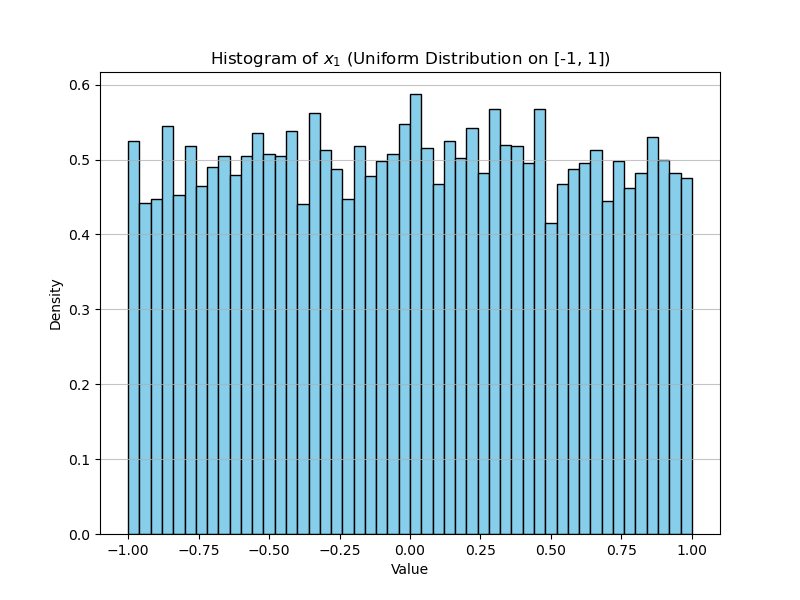
\includegraphics[width=0.8\textwidth]{./Figure_1.png}
    \caption{Histogram of the independently realized data for $x_1$ ($n=10,000$).}
    \label{fig:x1_hist}
	\end{figure}


	\textbf{Part (b)}\\
	Because $y_1$ depends exclusively on $\{x_1, x_2\}$ and $y_2$ depends exclusively on $\{x_3, x_4\}$, and the sets of variables are mutually independent, $y_1$ and $y_2$ are independent.\\
	The PDF of $x_i$ is $f_x(x) = \frac{1}{2}$ for $x \in [-1, 1]$.
	The PDF of $y_1 = x_1 + x_2$ is the convolution $f_x(y) * f_x(y)$. Convolving two identical rectangular pulses yields a triangular pulse:
	\[
		f_{y_1}(y) = f_{y_2}(y) = 
		\begin{cases}
			\frac{1}{4}(2 - |y|) & \text{for } |y| \le 2 \\
			0 & \text{otherwise}
		\end{cases}
	\]

	\textbf{Part (c)}\\
	$z = y_1 + y_2 = x_1 + x_2 + x_3 + x_4$.
	\begin{itemize}
	    \item \textbf{Mean:} $E[z] = \sum_{i=1}^4 E[x_i] = 4 \times 0 = 0$.
	    \item \textbf{Variance:} $\text{var}(z) = \sum_{i=1}^4 \text{var}(x_i)$. The variance of $U(-1,1)$ is $\frac{(1 - (-1))^2}{12} = \frac{1}{3}$. Thus, $\text{var}(z) = \frac{4}{3}$.
	    \item \textbf{PDF:} The PDF of $z$ is the convolution of two identical triangular distributions $f_z(z) = f_{y_1}(z) * f_{y_2}(z)$. The result is a scaled Irwin-Hall distribution ($n=4$) mapped to $[-4, 4]$:
	    \[
		f_z(z) = \frac{1}{96} \left[ (z+4)^3 U(z+4) - 4(z+2)^3 U(z+2) + 6z^3 U(z) - 4(z-2)^3 U(z-2) + (z-4)^3 U(z-4) \right]
	    \]
	\end{itemize}

	\textbf{Part (d)}\\
	We compare the empirical distribution of $z$ to a generated Normal distribution $N(0, 4/3)$. Because $z$ is the sum of 4 i.i.d. random variables, the Central Limit Theorem dictates that its distribution is already very close to Gaussian. The 2-sample Kolmogorov-Smirnov (KS) test evaluates the maximum distance between the empirical CDFs. Since $n=4$ approaches the normal distribution quite well, the test will typically yield a high p-value (e.g., $p > 0.05$), meaning we \textit{fail to reject} the null hypothesis. This empirically validates the Central Limit Theorem.
\end{proof}

\end{document}